% для компиляции в lualatex!!
\documentclass[12pt, a4paper]{article}
%\documentclass[12pt, a4paper]{disser}
\usepackage[english,russian]{babel}
\usepackage[warn]{mathtext}
\usepackage[T2A]{fontenc}
\usepackage[utf8]{inputenc}

%\usepackage{xecyr} % Продукт Вашего покорного слуги ;)

%\setmainfont{DejaVu Serif}
%\setmainfont{Liberation Serif}

\usepackage{color}
\usepackage{amssymb,amsmath}
\usepackage{graphicx}
\usepackage{multicol}

\textheight=24cm           % высота текста
\textwidth=16cm            % ширина текста
\oddsidemargin=0pt         % отступ от левого края
\topmargin=-1.5cm          % отступ от верхнего края
\parindent=24pt            % абзацный отступ
\parskip=0pt               % интервал между абзацами
\tolerance=2000            % терпимость к "жидким" строкам
\flushbottom               % выравнивание высоты страниц
%\def\baselinestretch{1.5} % печать с большим интервалом

%\title{}
%\author{\copyright~~С.А.~Назарова \thanks{e-mail:~sophia.nazarova@gmail.com}}
%\date{}


\begin{document}
	\begin{figure}[ht]
		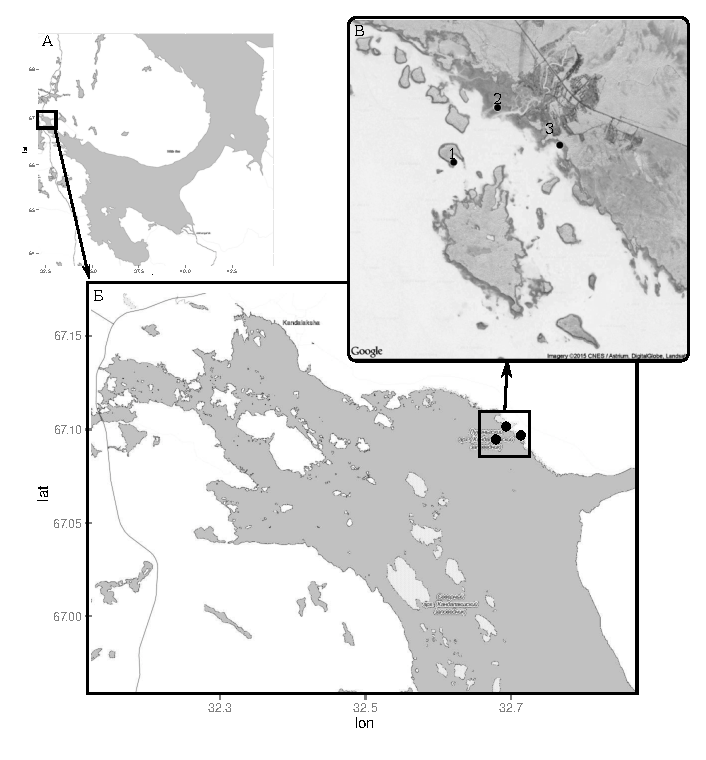
\includegraphics[height=0.45\textheight]{Nazarova_fig1.eps}	
	\end{figure}

	\begin{figure}[ht]
		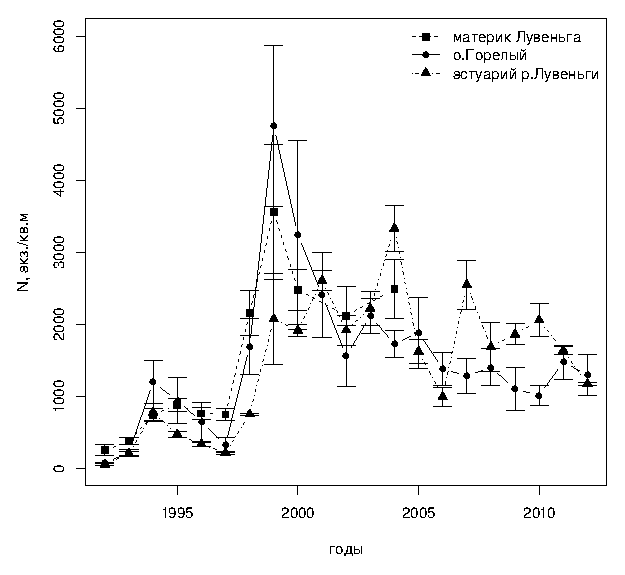
\includegraphics[height=0.45\textheight]{Nazarova_fig2.eps}	
	\end{figure}

	\begin{figure}[ht]
		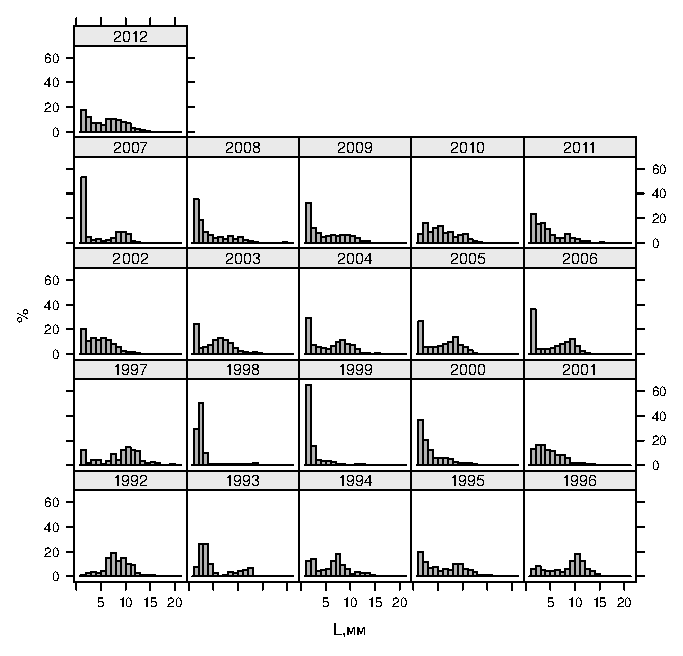
\includegraphics[height=0.45\textheight]{Nazarova_fig3.eps}	
	\end{figure}

	\begin{figure}[ht]
		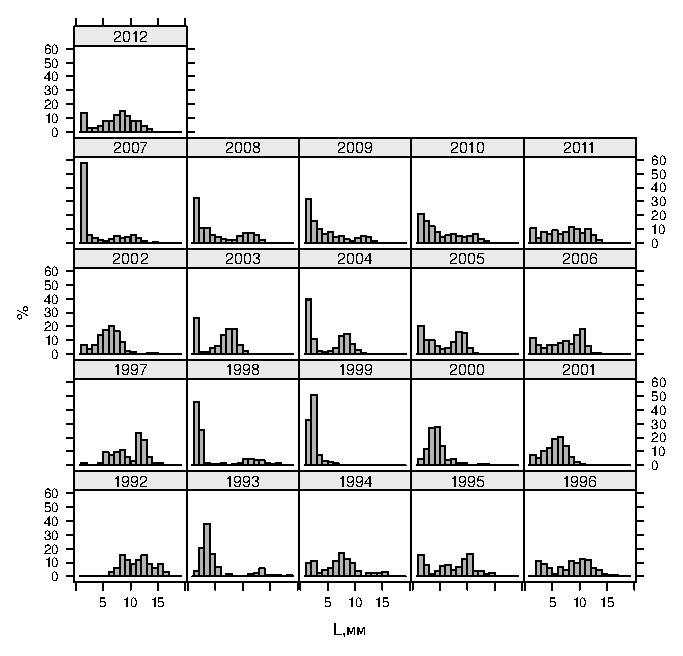
\includegraphics[height=0.45\textheight]{Nazarova_fig4.eps}	
	\end{figure}

	\begin{figure}[ht]
		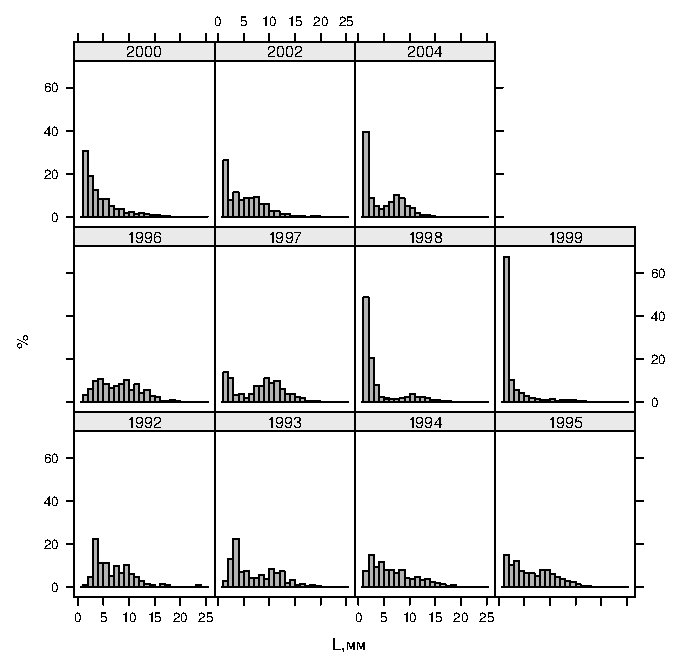
\includegraphics[height=0.45\textheight]{Nazarova_fig5.eps}	
	\end{figure}

	\begin{figure}[ht]
		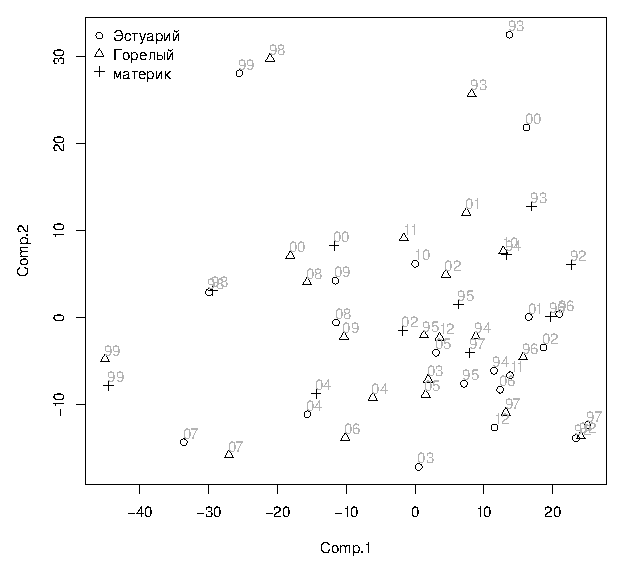
\includegraphics[height=0.45\textheight]{Nazarova_fig6.eps}	
	\end{figure}

	\begin{figure}[ht]
		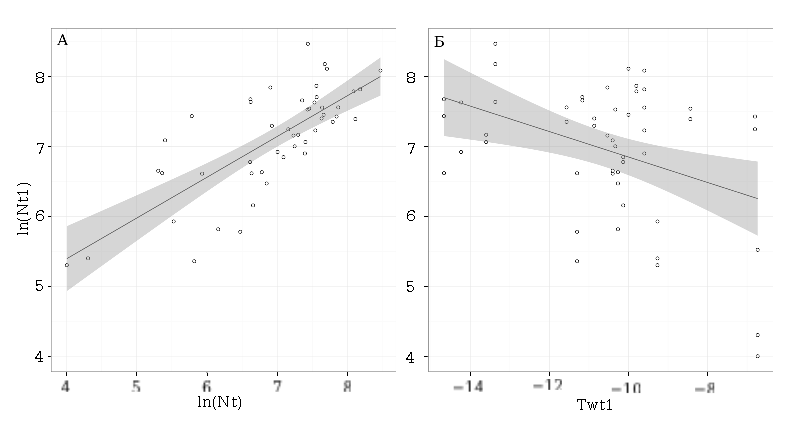
\includegraphics[width=\textwidth]{Nazarova_fig7.eps}	
	\end{figure}
\end{document}
